% ============================================== %
% PRELIMINARIES %
% ============================================== %

\begin{figure}
	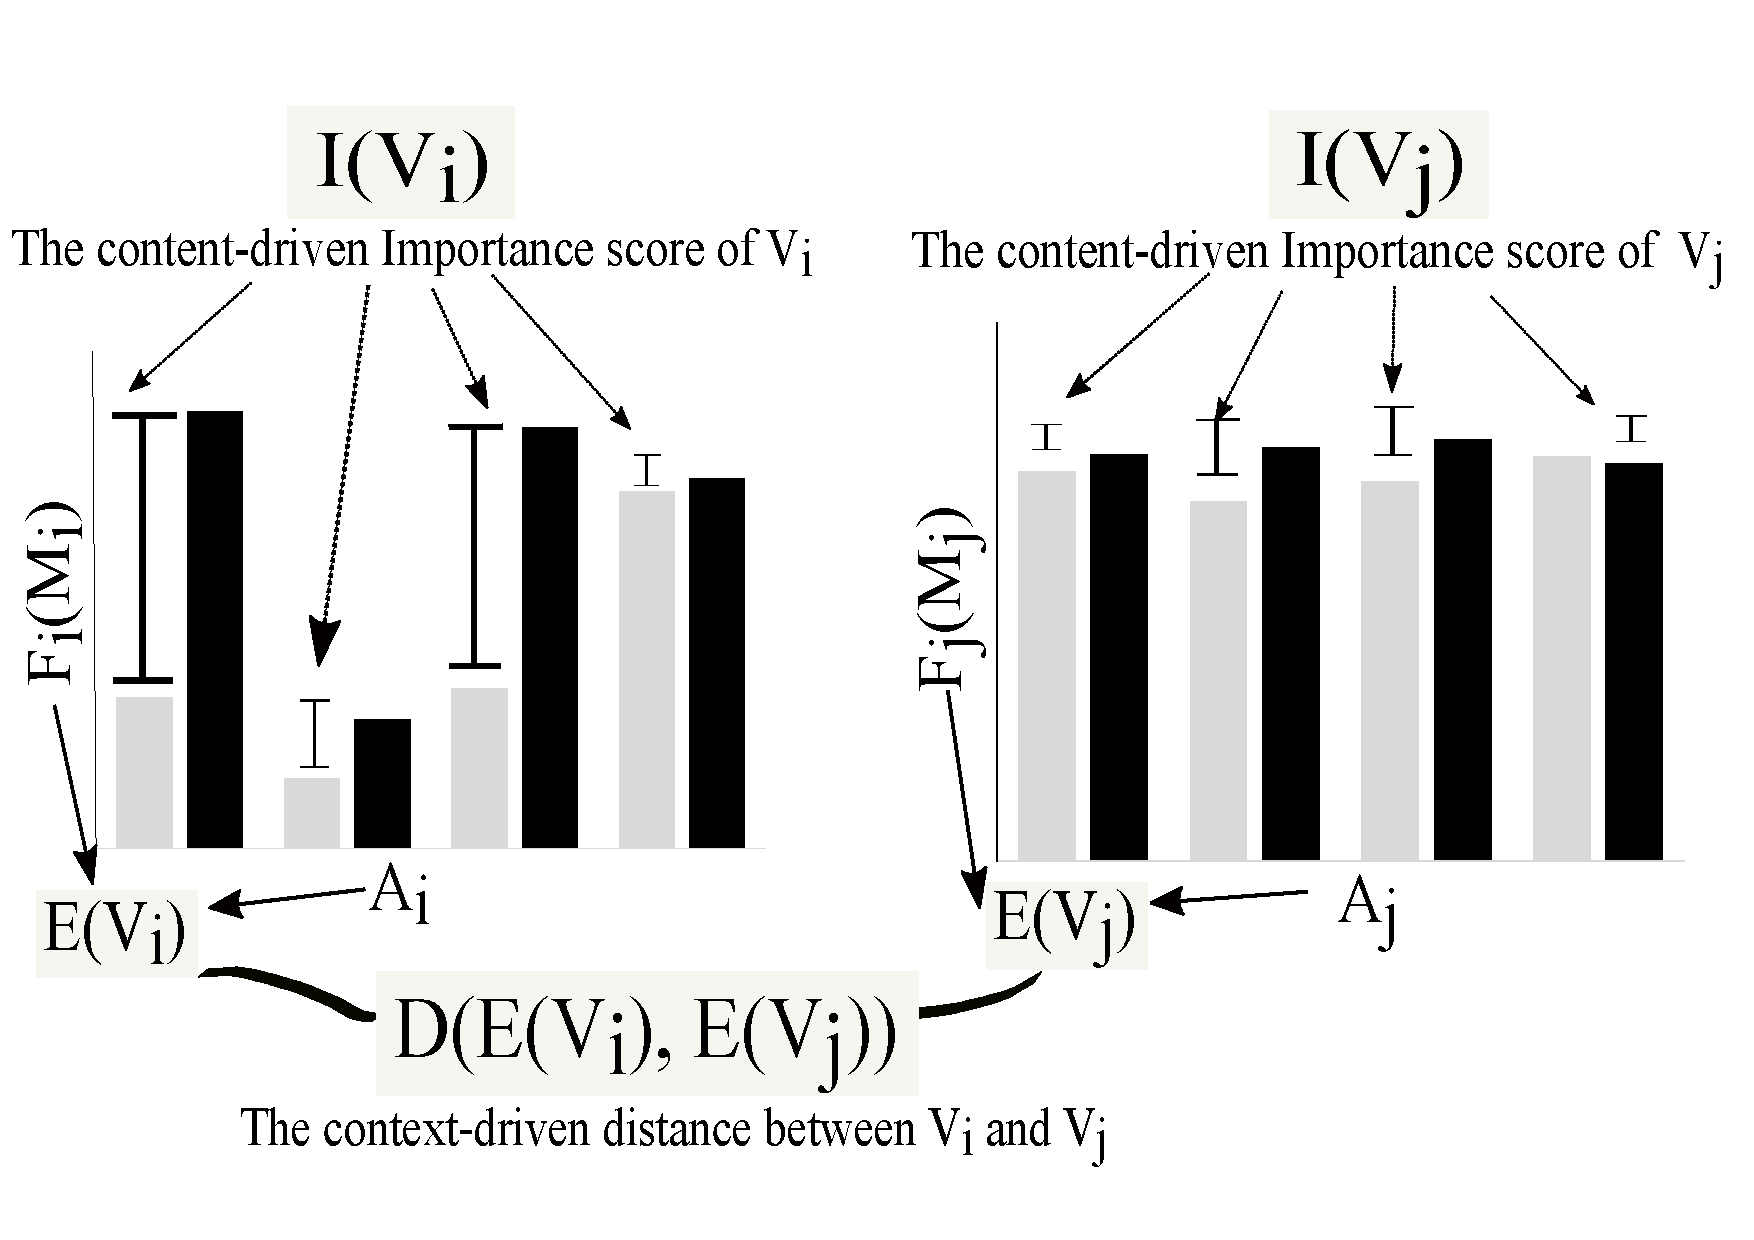
\includegraphics[width=3.5in,height=2.2in]{figures/introduction/pre2}
%	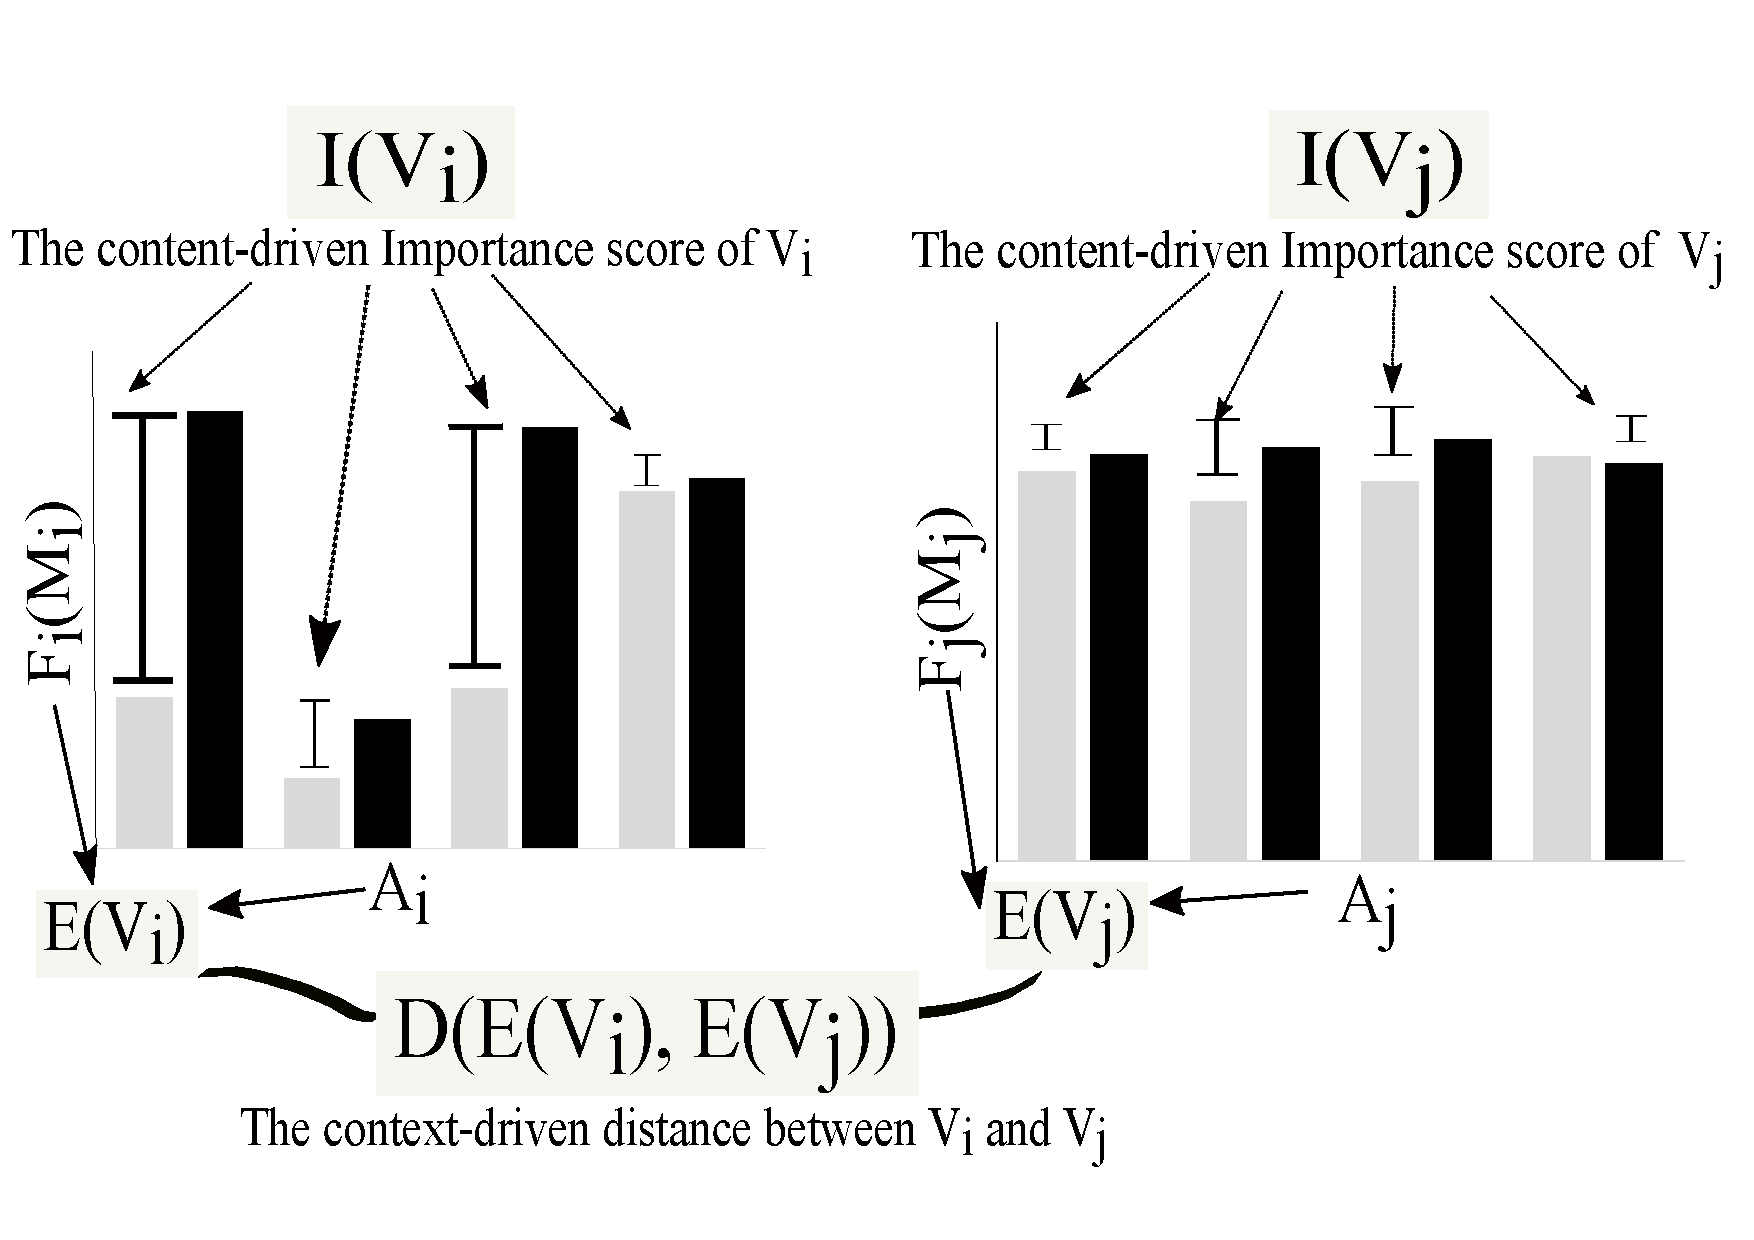
\includegraphics[width=4.5in,height=2.5in]{figures/introduction/pre2}
%	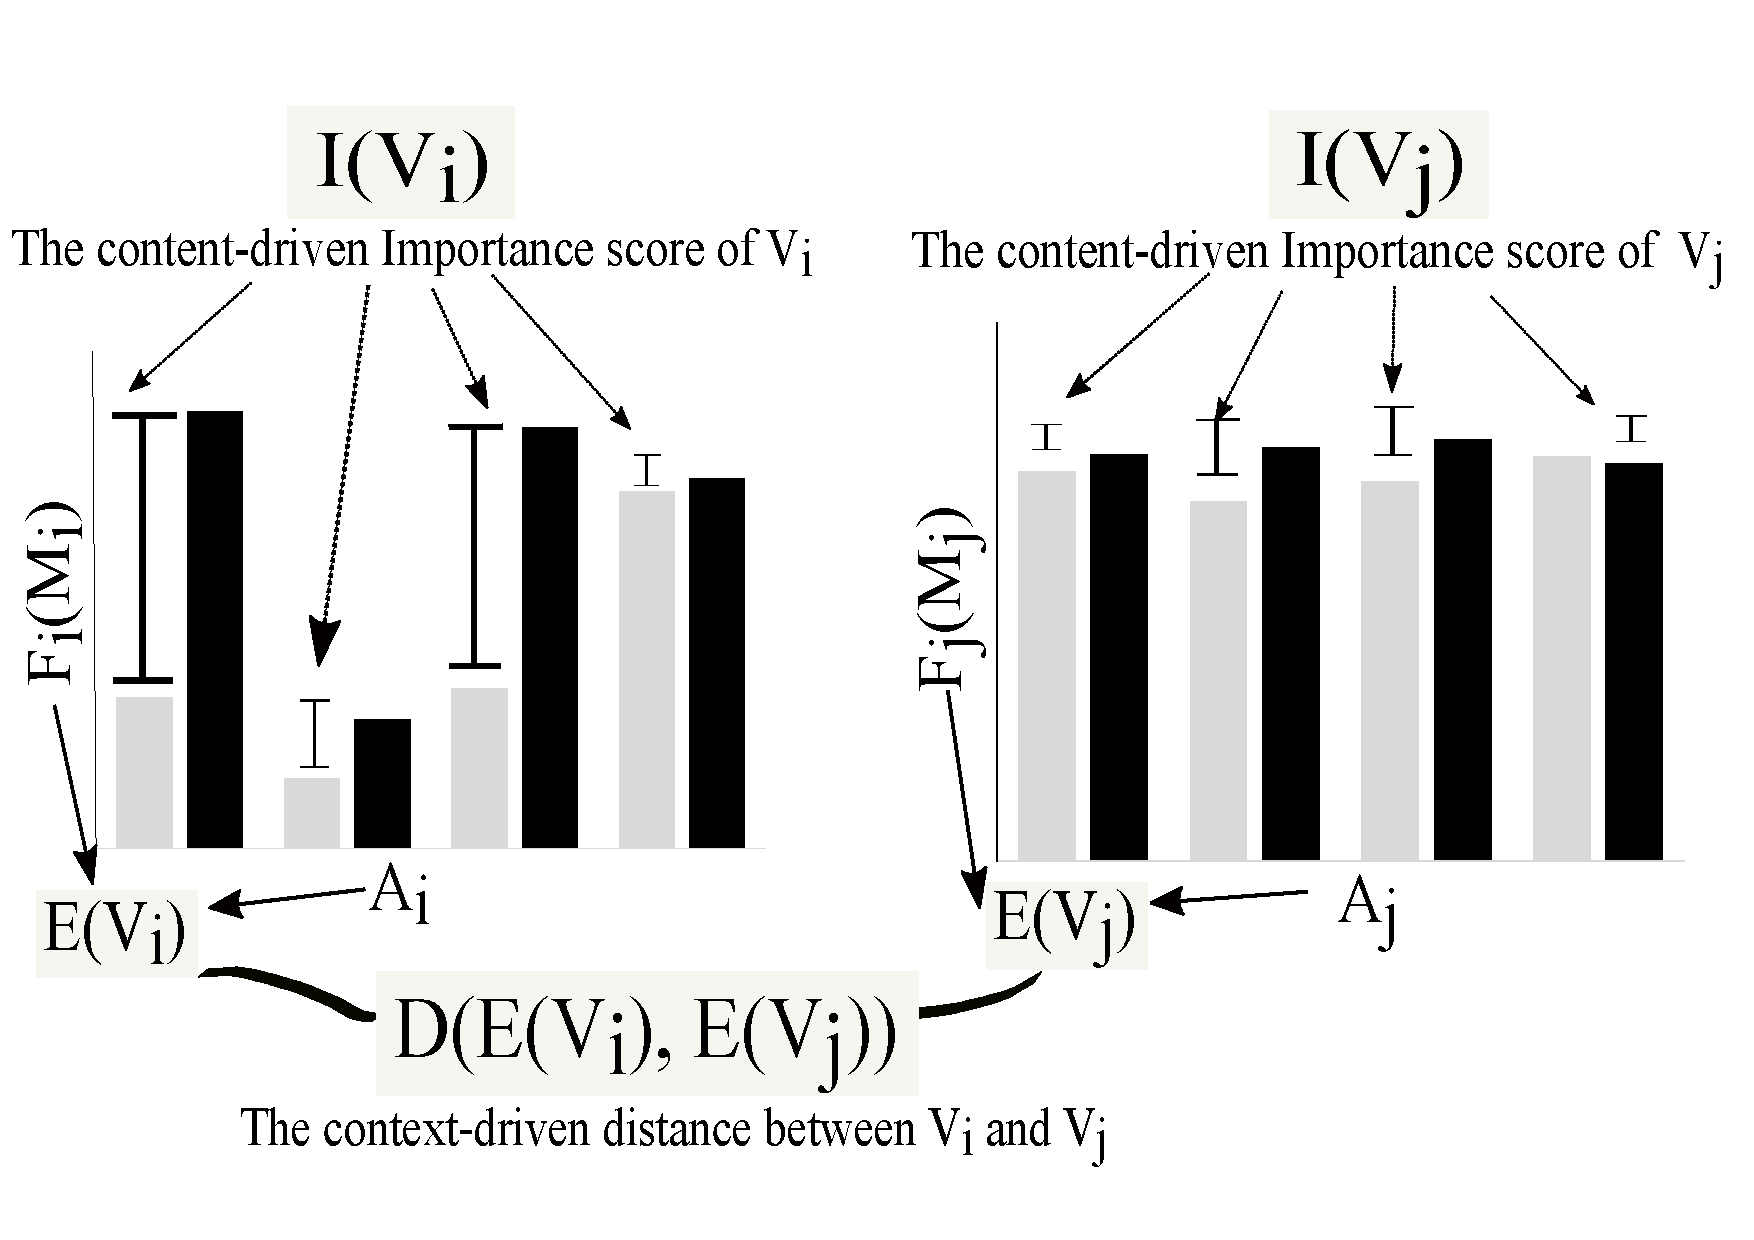
\includegraphics[width=5in]{figures/introduction/pre2}
\vspace{-18pt}
	\caption[content vs context]{Content vs. Context of views.}
	\label{fig:content-contex}
\vspace{-12pt}
\end{figure}

\section{Diversifying Recommended Views}
\label{sec:diversifying_recommended_visualizations}
% %

%\mas{short preamble}

Towards formulating our hybrid objective for view recommendation, in this section we describe the {\em content-based} deviation metric for assessing the importance of each view (Sec.~\ref{subsec:content_driven_deviation}), together with our {\em context-based} measure of the (dis)similarity between different views (Sec.~\ref{context-driven-deviation}). 
%
Those two metrics provide the foundations for our hybrid objective that aims to balance the tradeoff between importance and diversity in view recommendation (Sec.~\ref{subsec:problem_definition}).  
\vspace{-8pt}

\eat{
In order to diversifying recommended visualizations, we work at two levels. At the first level, content driven deviation metric is used to evaluate that how \quotes{important} is the content of the view as compared to the reference view. At the second level, we evaluate contextually how different a view is from other views in the recommended set using context driven deviation measure. The details of those two level are described next. 
}

\subsection{Content-Driven Importance}
\label{subsec:content_driven_deviation}

As  described in the previous section, we adopt a deviation-based metric to quantify the importance of a view \cite{Vartak2015,Vartak2014}. 
%
Essentially, the deviation-based metric compares an aggregate view generated from the selected subset dataset $D_Q$ (i.e., target view $V_i(D_Q)$) to the same view if generated from a reference dataset $D_R$ (i.e., reference view $V_i(D_R)$). 
%
%That reference dataset could be the whole database (i.e., $D_R=D_B$) or a selected subset of the database. 
%

Clearly, the deviation between a target and a reference view is a {\em data-driven} metric. 
%
That is, it measures the deviation between the {\em result} of $V_i(D_Q)$ and that of $V_i(D_R)$. 
%
Consequently, from a visualization point of view, that deviation is a {\em content-based} metric that captures the difference between the content of the visualization generated by $V_i(D_Q)$ vs. the visual content of  $V_i(D_R)$.
%
In the next, we formally describe the standard computation of that data-driven content-based metric, whereas the discussion of its counterpart context-driven metric is deferred to the next section.

To calculate the content-based deviation, each target view $V_i(D_Q)$ is normalized into a {\em probability distribution} $P[V_i(D_Q)]$ and similarly, each reference view into $P[V_i(D_R)]$.
%
In particular, consider an aggregate view $V_i=<\!A_i,M_i,F_i\!>$. 
%
The result of that view can be represented as the set of tuples: $<\!(a_j, g_j), (a_j, g_j), ..., (a_t, g_t)\!>$, where $t$ is the number of distinct values (i.e., groups) in attribute $A_i$, $a_j$ is the $j$-th group in attribute $A_i$, and $g_j$ is the aggregated value $F_i(M_i)$ for the group $a_j$ \cite{Ehsan2016, Vartak2015}. 
%
Hence, $V$ is normalized by the sum of aggregate values $G=\sum\limits_{j=1}^{t} g_j$, resulting in the probability distribution $P[V_i] = <\!\frac{g_1}{G}, \frac{g_2}{G}, ..., \frac{g_t}{G}\!>$.
%

Finally, the importance score of $V_i$ is measured in terms of the distance between $P[V_i(D_Q)]$ and $P[V_i(D_R)]$ (as illustrated in Figure~\ref{fig:content-contex}), and is simply defined as:
\begin{equation}
	I\left(V_i\right) = dist\left(P\left[V_i(D_Q)\right], P\left[V_i(D_R)\right]\right)
	\label{importance_score}
\end{equation}

\noindent where $ I\left(V_i\right) $ is the importance score of $ V_i$ and \textit{dist} is a distance function. 
%
Similar to existing work (e.g., \cite{Vartak2014,Vartak2015}), we adopt a Euclidian distance, but other distance measures are also applicable (e.g., Earth Mover's distance, K-L divergence, etc.). 

In current approaches for view recommendation, the importance value $I(V_i)$ of each possible view $V_i$ is computed, and the $k$ views with the highest deviation are recommended.
%
However, in this work, our goal is to ensure that recommended views provide a good coverage of possible insights, which is described next. 
\vspace{-2pt}
\subsection{Context-Driven Similarity}
\label{context-driven-deviation}
% % Prolog 

As mentioned above, recommending views based only on their data content often leads to a set of similar views. 
%
In order to provide full coverage of all possible interesting insights, in this work, we posit that achieving {\em diversity} within the set of recommended views is an essential quality measure. 
%
%Diversity has been well known and widely used in recommendation systems for maximizing information gain and minimizing redundancy (e.g., \cite{Zhang2008, Rafiei2010, Yu2009, Vieira2011}). 
%
%At a high level, diversity essentially measures how different (i.e., diverse) are the individual data objects within a set. 
%	
Before discussing the details of diversity computation in Sec.~\ref{subsec:problem_definition}, it is important to notice that central to that computation is some notion of distance measure between data objects.
%
Existing work provides multiple metrics for measuring that distance between traditional data objects, such as web documents (e.g., \cite{Rafiei2010,Clarke2008,Zhang2008}), database tuples (e,g, \cite{DBLP:conf/sigmod/TranC10}), etc.
%
However, our work in this paper is the first to consider diversity in the context of aggregate data visualizations. 
%
As such, a metric is needed to quantify the (dis)similarity between the distinct features of different visualizations.
%
Towards this, we re-emphasize that each visualization is merely a data view generated by an aggregate query. 
%
Thus, such metric naturally lends itself to considering the query underlying each view (i.e., the query  executed to create the view). 
%
In turn, the distance between two views is measured based on the distance between their underlying queries.  
%
Hence, in addition to our data-driven content-based deviation, we also introduce a query-driven {\em context-based} deviation metric.
%
 Figure~\ref{fig:content-contex} illustrates and summarizes our proposed metrics.
	


%To measure the context-based deviation between two visualizations, we simply measure the distance between their underlying queries. 
%
Towards measuring the context-based deviation, we extend on existing work in the area of query recommendation and refinement (e.g., \cite{DBLP:conf/sigmod/TranC10,DBLP:conf/dexa/Kantere16,DBLP:conf/cikm/KantereOKS15}).
%
In that work, the distance between two range queries $q_1$ and $q_2$ is mapped to that of measuring the edit distance needed to transform $q_1$ into $q_2$. %where the set of allowed transformation are: add, delete, or modify a predicate. 
%
In the context of our work, however, views are generated from aggregate queries without range predicates. 
%
In particular, a view is fully defined in terms of a combination of attribute, measure and an aggregate function.
%
Hence, in addition to the content of a view $V_i$ which is described by its probability distribution (i.e., $P(V_i))$ as defined in Sec. ~\ref{subsec:content_driven_deviation}), we also consider the context of the view $E(V_i)$, which is defined in terms of the query underlying $V_i$ as:
%
$E(V_{i})=  \{A_i, M_i, F_i\}$.




Such definition of view context leads to a special case of the existing work on query recommendation, in which the normalized distance between two queries is simply measured using the {\em Jaccard} similarity measure.
%
Hence, the Jaccard similarity between two aggregate views $V_i$ and $V_j$ is measured as: $ J(V_{i}, V_{j} ) = \dfrac{| E(V_{i}) \cap E(V_{j}) |}{| E(V_{i}) \cup E(V_{j})|} $	
%\note{update figure to reflect all those changes here and also check all equations for mistakes while making the changes}
%done

We note that the jaccard similarity assigns equal weights to each of the element in a set. 
%
Accordingly, when applied to aggregate views, then two views with the same attribute and different measure and aggregate function will have the same similarity score as any other pair of views with same measure but different attribute and aggregate function. 
%
However, an analyst may consider two views with the same attribute $A_i$ more similar than two views with same measure attribute $M_i$. 
%
To allow the analyst to specify such preference, each contextual component of a view is associated with a weight that specifies its impact on determining the (dis)similarity between views. 
%
Specifically, let $w_i$ be the weight assigned to $i^{th}$ element of set $E(V_i)$, where $\sum_{i=1}^{3}w_i =1$.
%
Then, the similarity between views $V_i$ and $V_j$ is measured as: $J(V_{i}, V_{j} ) = \dfrac{\sum_{i\in V_i \cap V_j}w_i}{\sum_{i\in V_i \cup V_j}w_i} $
%	
Consequently, the context-based deviation between $V_i$ and $V_j$ is calculated as:
\vspace{-4pt}
\begin{equation}
D\left(V_{i}, V_{j} \right) = 1- J\left(V_{i}, V_{j} \right) 
\label{diversity_score}                 
\end{equation}
\vspace{-14pt}



%
\eat{
Particularly, it shows two views $V_i$ and $V_j$, for which the content-driven importance values $I(V_i)$ and $I(V_j)$ are computed based on the probability distribution of the data in each view. 
%
Moreover, it also shows the context-driven distance between those two views, which is computed as $D\left(V_{i}, V_{j} \right)$. 
}

\eat{
% %
As a summarize, the difference betweeen content and context of view is described in Figure \ref{fig:content-contex}.
% %
Content is the probability distribution of the aggregated query result, whereas, Context is described as a set containing the name of the attribute, measure and function used to generate the view.  
% %
		}

\eat{
Thus, in the process to recommend users a set of top-k views, we work at two levels.
% %
At the first level, we evaluate that how \quotes{important} is the content of the view as compared to the reference view using content driven deviation metric. 
%In particular, we determine how different are the trends and patterns revealed by $V_{T}$ from its reference $V_{R}$ in terms of content. 
% %
At the second level, we evaluate contextually how different a view is from other views in the recommended set using context driven deviation measure. 
% %
}


%
%
%% %
%The difference betweeen content and context is described in Figure \ref{fig:pre}.
%% %
%Content as in Figure \ref{fig:pre1} is the probability distribution of the aggregated query result, whereas, Context as in Figure \ref{fig:pre2} is described as a set containing the name of the attribute, measure and function used to generate the view.  
%
%% %
